\documentclass{beamer}
\mode<presentation>
\usetheme{CambridgeUS}
\usepackage[russian]{babel}
\usepackage[utf8]{inputenc}
\usepackage[T2A]{fontenc}
\usepackage{sansmathaccent}

\usepackage{verbatim}
\usepackage{alltt}

\pdfmapfile{+sansmathaccent.map}
\title[Шаблоны]{Шаблоны информационной архитектуры}
\author{Наумов Д.А., доц. каф. КТ}
\date[18.11.2020] {Компьютерная графика и проектирование графических интерфейсов, 2020}

\begin{document}

%ТИТУЛЬНЫЙ СЛАЙД
\begin{frame}
  \titlepage
\end{frame}
  
%СОДЕРЖАНИЕ ЛЕКЦИИ
\begin{frame}
  \frametitle{Содержание лекции}
  \tableofcontents  
\end{frame}

\section{Информационная архитектура}

\begin{frame}[t]
	Высокоуровневая оганизация информации:
	\begin{itemize}
		\item разделение сущностей -- отделение содержимого от физического представления;
		\item физическая структура -- представление материала на страницах.
	\end{itemize}
	
	Большинство приложений и многие веб-сайты организуются соглласно одному из нескольких следующих принципов:
	\begin{itemize}
		\item списки объектов -- папка входящих сообщений;
		\item списки действий или задач -- посмотреть, приобрести, продать, зарегистрироваться; 		
		\item списки тематических категорий -- здоровье, наука, технология;		
		\item списки инструментов -- календарь, адресная книга, блокнот.		
	\end{itemize}
	
	Любую страницу можно рассматривать с точки зрения того, что оно долнжа делать:
	\begin{itemize}
		\item отобразить едиственный объект (карта, книга, видео, игра);
		\item отобразить список объектов;
		\item предоставить возможность что-то сделать;
		\item выполнить определенную задачу.				
	\end{itemize}	

\end{frame} 

\begin{frame}[t]{Feature, Search and Browse}
	Расположите на главной странице три элемента: статья-описание, поиск и список категорий для навигации.
	\begin{figure}[h]
		\centering
		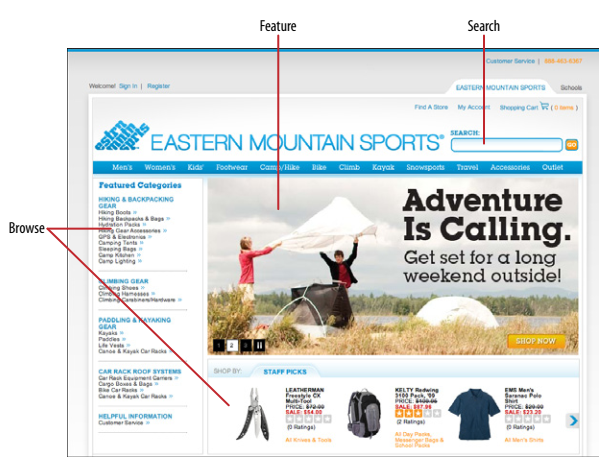
\includegraphics[scale=0.5]{images/lec07-pic01.png}
	\end{figure}
\end{frame} 

\begin{frame}[t]{Feature, Search and Browse}
	\begin{figure}[h]
		\centering
		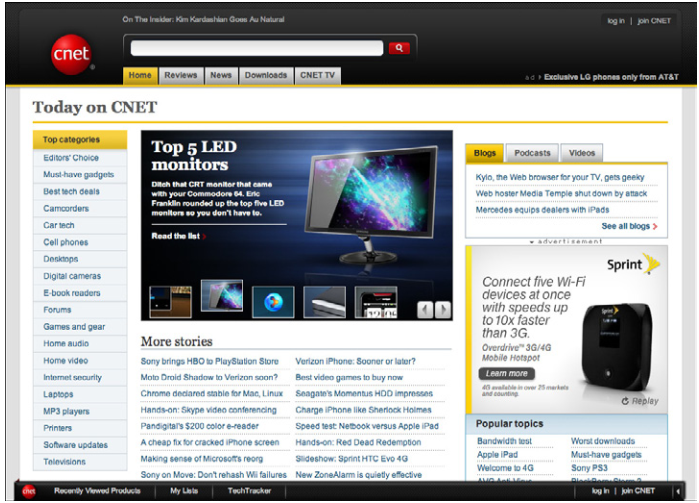
\includegraphics[scale=0.5]{images/lec07-pic02.png}
	\end{figure}
\end{frame} 

\begin{frame}[t]{News Stream}
	Отобразите элементы в обратном хронологическом порядке, обновляйте их динамически.
	\begin{figure}[h]
		\centering
		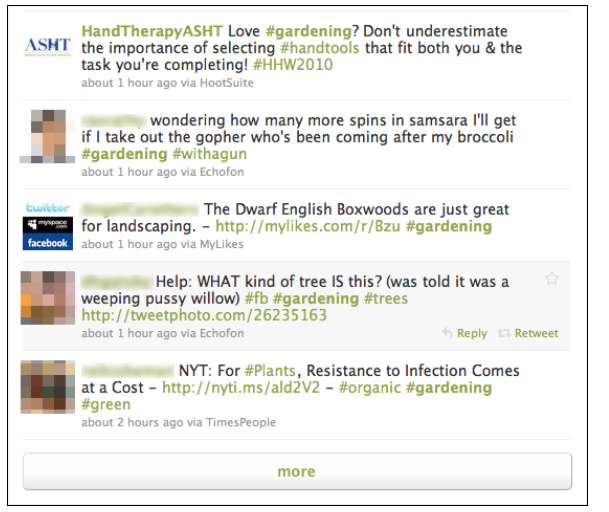
\includegraphics[scale=0.5]{images/lec07-pic04.png}
	\end{figure}
\end{frame} 

\begin{frame}[t]{Picture Manager}
	Используйте эскизы, список элементов и интерфейс просмотра.
	\begin{figure}[h]
		\centering
		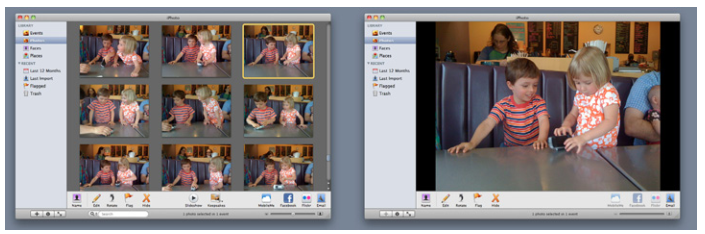
\includegraphics[scale=0.6]{images/lec07-pic06.png}
	\end{figure}
\end{frame} 

\begin{frame}[t]{Dashboard}
	Организуйте отображение данных в единую информационную страницу, регулярно обновляемую. Покажите пользователям релевантную, полезную информацию и позвольте им настроить дисплей по мере необходимости.
	\begin{figure}[h]
		\centering
		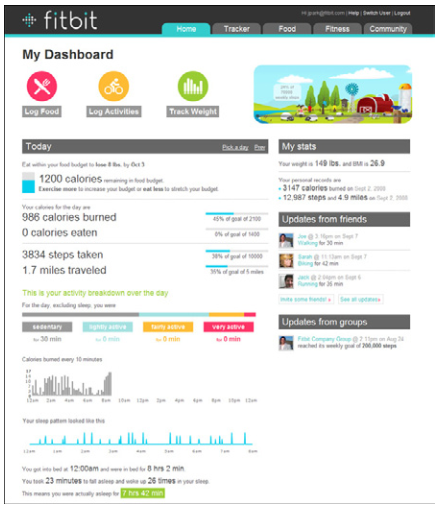
\includegraphics[scale=0.6]{images/lec07-pic08.png}
	\end{figure}
\end{frame} 

\begin{frame}[t]{Canvas plus Palette}
	Поместите палитру рядом с холстом; пользователь сможет выбирать инструменты на палитры, чтобы создать объекты на холсте.
	\begin{figure}[h]
		\centering
		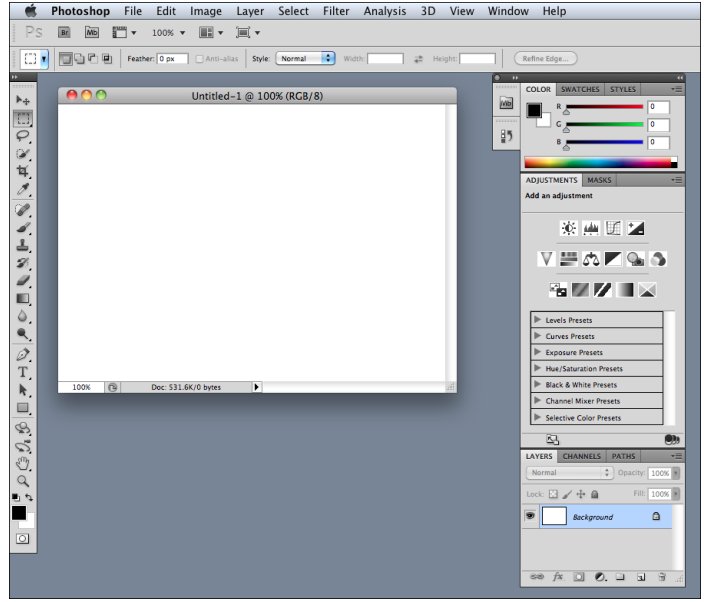
\includegraphics[scale=0.6]{images/lec07-pic09.png}
	\end{figure}
\end{frame} 

\begin{frame}[t]{Wizard}
	Проведите пользователя через интерфейс шаг за шагом, чтобы выполнить задачи в заданном порядке.
	\begin{figure}[h]
		\centering
		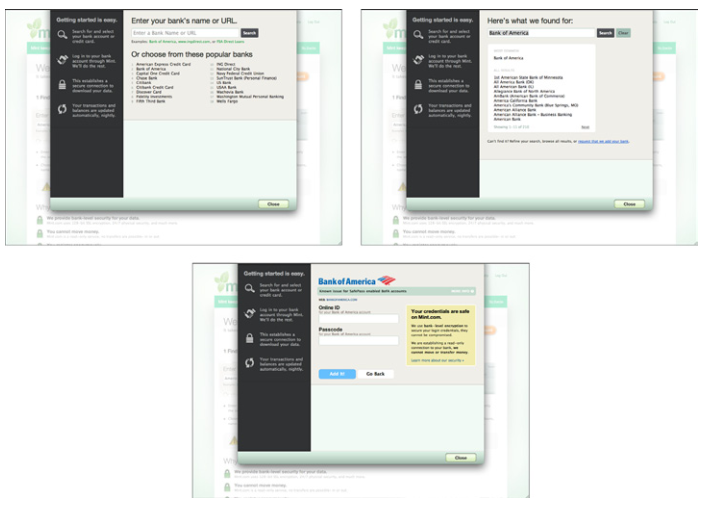
\includegraphics[scale=0.6]{images/lec07-pic10.png}
	\end{figure}
\end{frame} 

\begin{frame}[t]{Settings}
	Предоставьте легкодоступную страницу, где пользователи могут изменять настройки,
предпочтения или свойства. Разделите содержимое на отдельные вкладки или страницы, если вам нужно управлять большим количеством настроек.
	\begin{figure}[h]
		\centering
		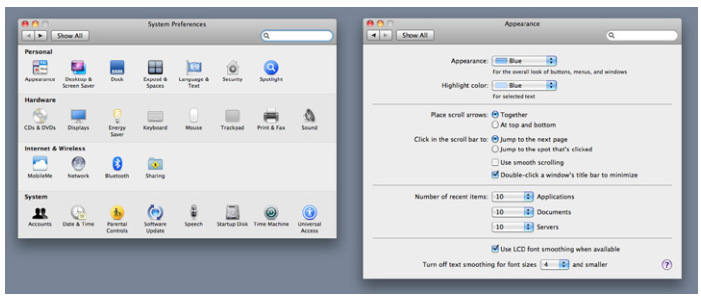
\includegraphics[scale=0.6]{images/lec07-pic11.png}
	\end{figure}
\end{frame} 

\begin{frame}[t]{Alternative Views}
	Позвольте пользователю выбирать один из альтернативных вариантов, существенно отличающихся от вида по умолчанию.
	\begin{figure}[h]
		\centering
		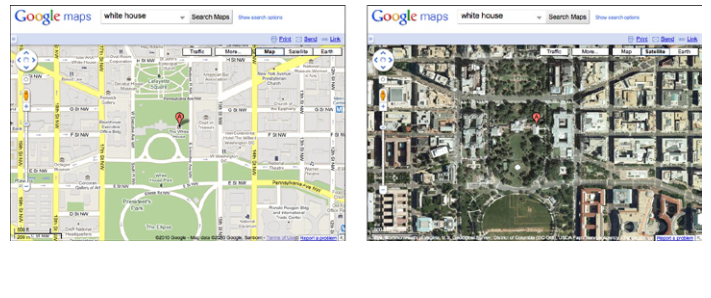
\includegraphics[scale=0.6]{images/lec07-pic12.png}
	\end{figure}
\end{frame} 

\begin{frame}[t]{Many Workspaces}
	Используйте несколько вкладок верхнего уровня, групп вкладок и окон, чтобы пользователи могли одновременно просматривать несколько страниц, проектов, файлов или контекстов. 
	\begin{figure}[h]
		\centering
		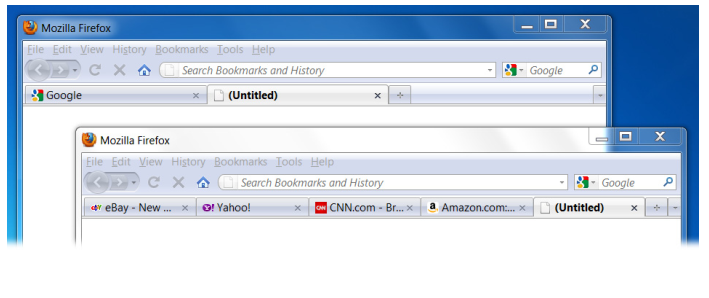
\includegraphics[scale=0.6]{images/lec07-pic13.png}
	\end{figure}
\end{frame}

\begin{frame}[t]{Multi-level Help}
	Используйте различные варианты помощи и подсказок для поддержки пользователей с различными потребностями. 
	\begin{figure}[h]
		\centering
		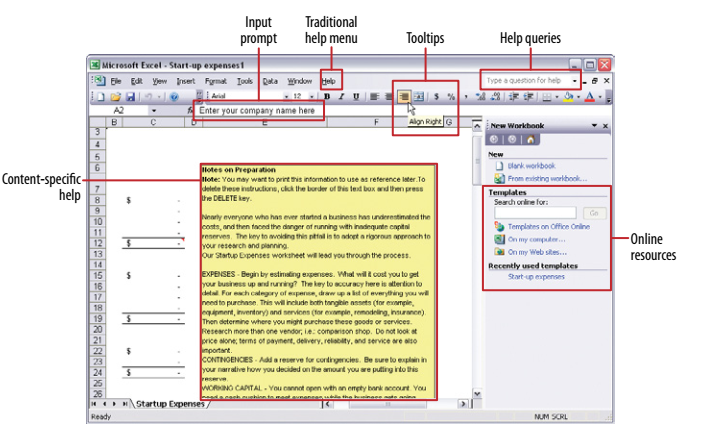
\includegraphics[scale=0.5]{images/lec07-pic14.png}
	\end{figure}
\end{frame}

\section{Навигация}

%СОДЕРЖАНИЕ ЛЕКЦИИ
\begin{frame}
  \frametitle{Содержание лекции}
  \tableofcontents[current]
\end{frame}

\begin{frame}[t]
	Указатели (signpost) -- средства, позволяющие пользователям ориентироваться на стренице.
	\begin{itemize}
		\item заголовки (страниц, окон);
		\item логотипы;
		\item вкладки;
		\item индикаторы выбора и т.д.						
	\end{itemize}
	
	Указатели:
	\begin{itemize}
		\item ясные и недвусмысленные;
		\item расположены в ожидаемом месте;
		\item создают правильную <<ментальную карту>> сайта.
	\end{itemize}
	
	Цена навигации: сколько сил потратит пользователь, чтобы соориентироваться на новой странице.
	
	Задача построения системы навигации -- минимизация количества переходов пользователя для достижения его целей.
\end{frame} 

\begin{frame}[t]
	Глобальная навигация -- находится на каждом главном экране, принимает форму
меню, вкладок и/или боковых панелей, и именно так пользователи перемещаются по формальной навигационной структуре сайта. 
	Вспомогательная навигация --  содержит ссылки и инструменты, связанные с
неконтентными аспектами сайта или приложения: вход, справка, печать, редакторы настроек, языковые средства и т. д.
	Ассоциативная навигация встраивает ссылки в фактическое содержимое или рядом с ним. Когда пользователь читает или взаимодействует с сайтом, эти ссылки представляют варианты, которые могут быть немедленно актуальны для пользователя. Они связывают содержание воедино тематически.
\end{frame} 

\begin{frame}[t]{Clear Entry Points}
	Представьте только несколько основных точек входа в интерфейс; сделайте их ориентированными на задачи и описательными. Используйте четкие призывы к действию. 
	\begin{figure}[h]
		\centering
		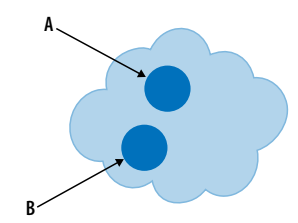
\includegraphics[scale=0.5]{images/lec07-pic23.png}
	\end{figure}
\end{frame}

\begin{frame}[t]{Clear Entry Points}
	\begin{figure}[h]
		\centering
		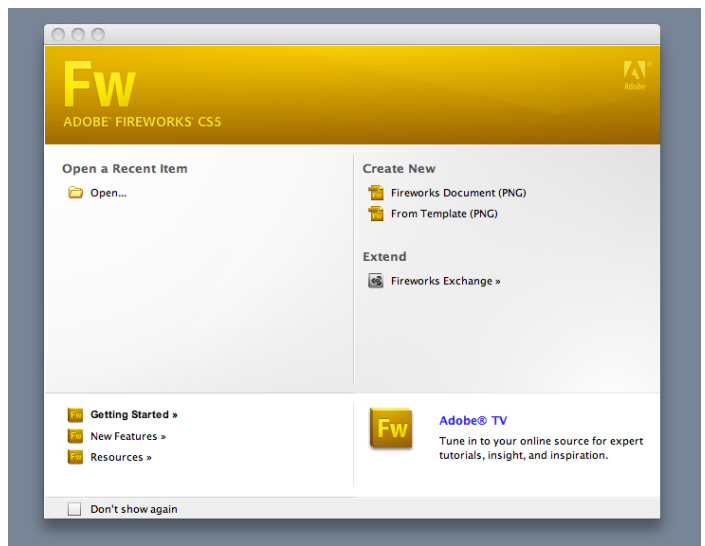
\includegraphics[scale=0.5]{images/lec07-pic24.png}
	\end{figure}
\end{frame}

\begin{frame}[t]{Main Page}
	Заполните страницу списком ссылок на содержательные страницы вашего сайта или приложения. Покажите достаточно информации о каждой ссылке, чтобы пользователь мог сделать правильный выбор. Не показывайте на странице никакого другого значимого
контента. 
	\begin{figure}[h]
		\centering
		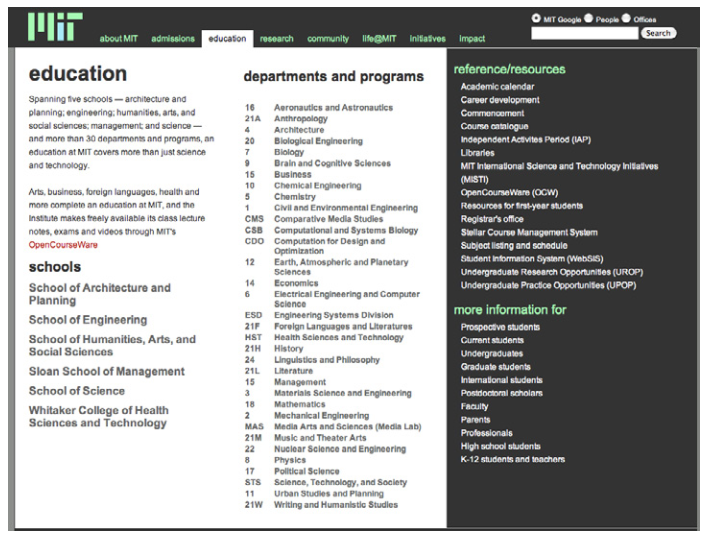
\includegraphics[scale=0.5]{images/lec07-pic26.png}
	\end{figure}
\end{frame}

\begin{frame}[t]{Main Page}
	\begin{figure}[h]
		\centering
		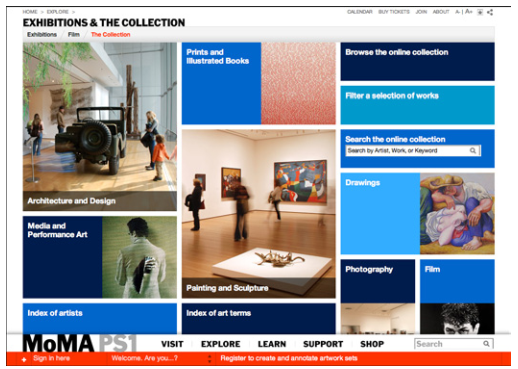
\includegraphics[scale=0.5]{images/lec07-pic27.png}
	\end{figure}
\end{frame}

\begin{frame}[t]{Pyramid}
	Создайте последовательность страниц с ссылками prev/next. Создайте родительскую страницу, которая ссылается на все страницы в этой последовательности, и позвольте пользователю просматривать их либо последовательно, либо в произольном порядке. 
	\begin{figure}[h]
		\centering
		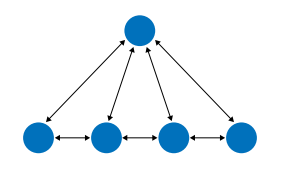
\includegraphics[scale=0.5]{images/lec07-pic28.png}
	\end{figure}
\end{frame}

\begin{frame}[t]{Pyramid}
	\begin{figure}[h]
		\centering
		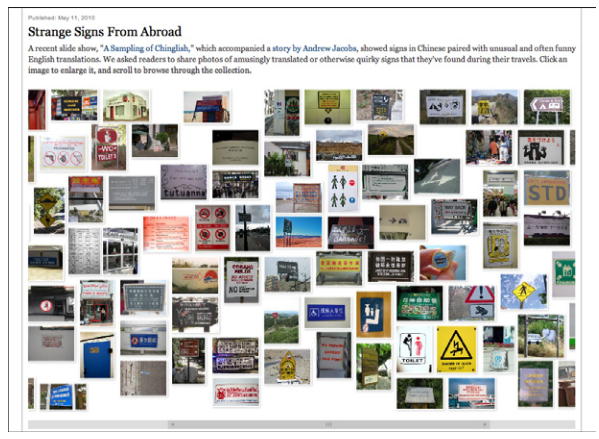
\includegraphics[scale=0.3]{images/lec07-pic29.png}
	\end{figure}
	\begin{figure}[h]
		\centering
		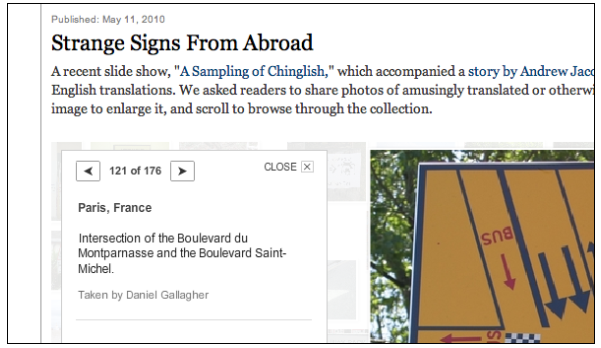
\includegraphics[scale=0.3]{images/lec07-pic30.png}
	\end{figure}
\end{frame}

\begin{frame}[t]{Modal Panel}
	Отображайте только одну страницу без каких-либо других параметров навигации, пока пользователь не выполнит ближайшую задачу. 
	\begin{figure}[h]
		\centering
		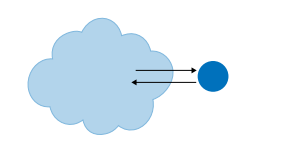
\includegraphics[scale=0.5]{images/lec07-pic31.png}
	\end{figure}
\end{frame}

\begin{frame}[t]{Modal Panel}
	\begin{figure}[h]
		\centering
		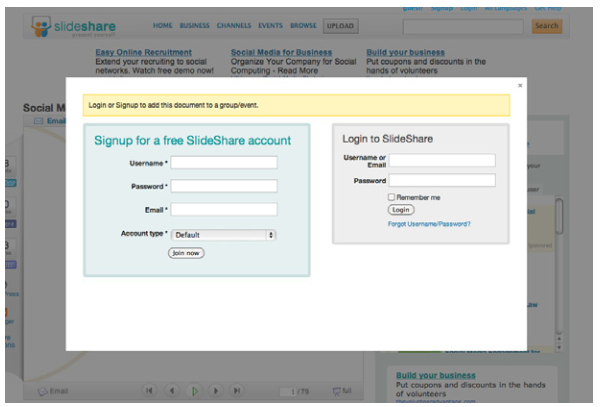
\includegraphics[scale=0.5]{images/lec07-pic32.png}
	\end{figure}
\end{frame}

\begin{frame}[t]{Deep-linked state}
	Зафиксируйте состояние сайта в URL-адресе, который можно сохранить или отправить другим людям. При загрузке он восстанавливает состояние приложения до того, что видел пользователь. 
	\begin{figure}[h]
		\centering
		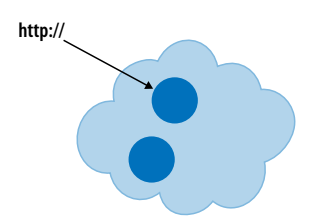
\includegraphics[scale=0.5]{images/lec07-pic33.png}
	\end{figure}
\end{frame}

\begin{frame}[t]{Deep-linked state}
	\begin{figure}[h]
		\centering
		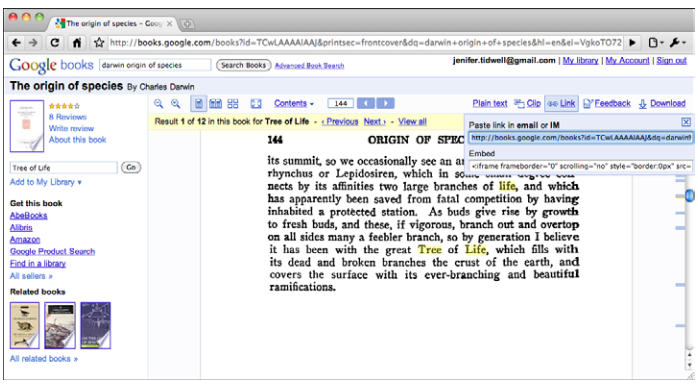
\includegraphics[scale=0.5]{images/lec07-pic34.png}
	\end{figure}
\end{frame}

\begin{frame}[t]{Escape Hatch}
	На каждом экране, имеющем ограниченные возможности навигации, поместите кнопку или ссылку, которая явно выводит пользователя из этого экрана и возвращает в известное место. 
	\begin{figure}[h]
		\centering
		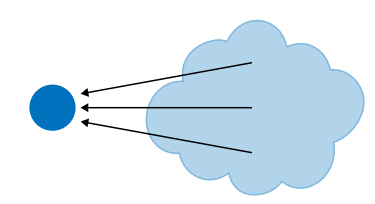
\includegraphics[scale=0.5]{images/lec07-pic35.png}
	\end{figure}
\end{frame}

\begin{frame}[t]{Escape Hatch}
	\begin{figure}[h]
		\centering
		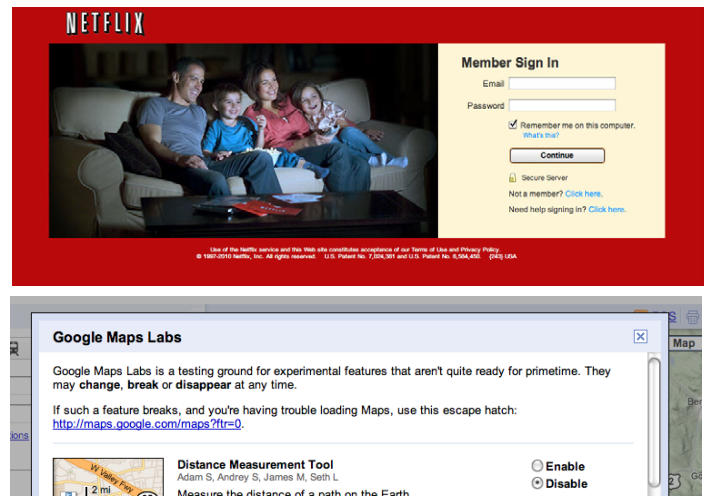
\includegraphics[scale=0.5]{images/lec07-pic36.png}
	\end{figure}
\end{frame}	

\begin{frame}[t]{Fat Menus}
	Для длинного списка навигационных ссылок используйте меню. Используйте хорошо подобранные категории или естественный порядок сортировки.
	\begin{figure}[h]
		\centering
		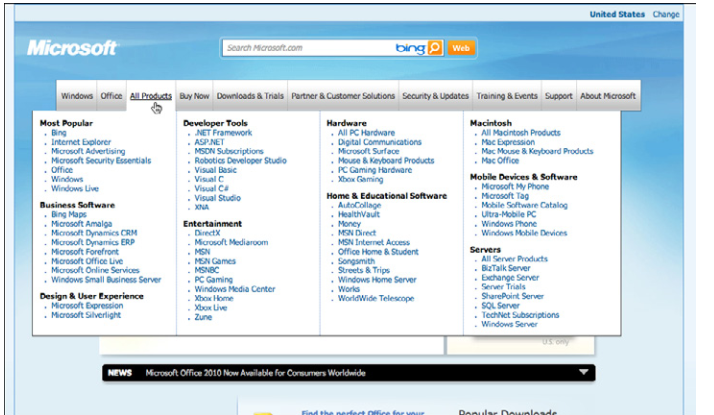
\includegraphics[scale=0.5]{images/lec07-pic37.png}
	\end{figure}
\end{frame}	

\begin{frame}[t]{Fat Menus}
	\begin{figure}[h]
		\centering
		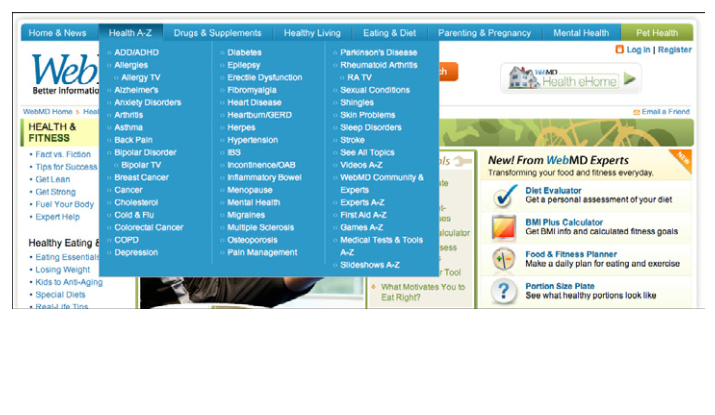
\includegraphics[scale=0.5]{images/lec07-pic38.png}
	\end{figure}
\end{frame}	

\begin{frame}[t]{Sitemap Footer}
	Поместите карту сайта в нижний колонтитул каждой страницы сайта. Рассматривайте его как часть глобальной навигации, дополняющую заголовок.
	\begin{figure}[h]
		\centering
		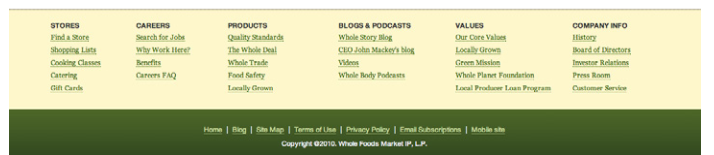
\includegraphics[scale=0.5]{images/lec07-pic39.png}
	\end{figure}
	\begin{figure}[h]
		\centering
		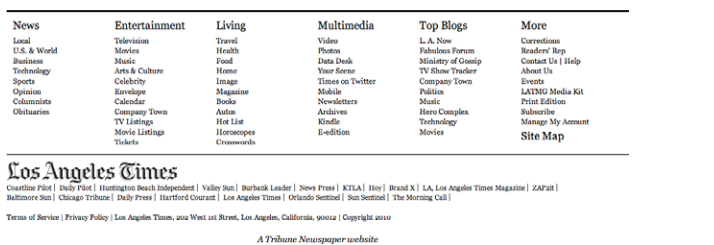
\includegraphics[scale=0.5]{images/lec07-pic41.png}
	\end{figure}	
\end{frame}	

\begin{frame}[t]{Sitemap Footer}
	\begin{figure}[h]
		\centering
		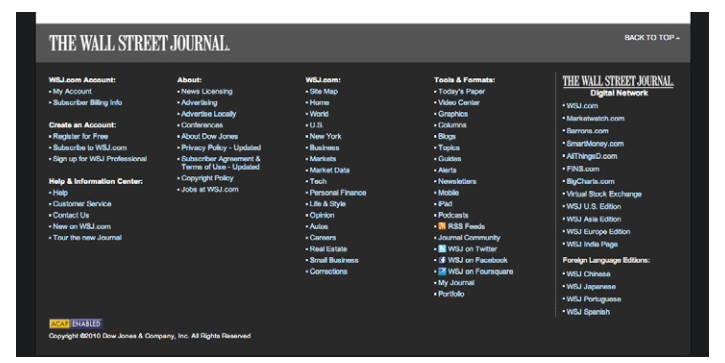
\includegraphics[scale=0.5]{images/lec07-pic40.png}
	\end{figure}	
\end{frame}	

\begin{frame}[t]{Sign-in Tools}
	Поместите служебную навигацию, связанную с регистрацией/авторизацией пользователя, в правый верхний угол. Там же расположите корзины, ссылки на настройку профиля и учетной записи, кнопки справки и выхода из системы.
	\begin{figure}[h]
		\centering
		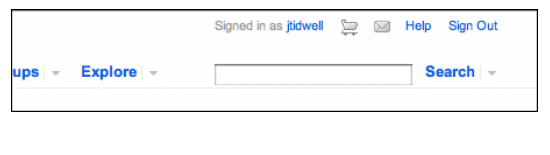
\includegraphics[scale=0.5]{images/lec07-pic42.png}
	\end{figure}
\end{frame}	

\begin{frame}[t]{Sequence Map}
	На каждой странице из определенной последовательности покажите карту всех страниц по порядку, включая индикатор <<вы находитесь здесь>>.
	\begin{figure}[h]
		\centering
		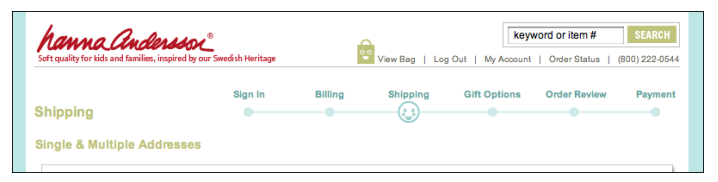
\includegraphics[scale=0.5]{images/lec07-pic43.png}
	\end{figure}
\end{frame}	

\begin{frame}[t]{Sequence Map}
	\begin{figure}[h]
		\centering
		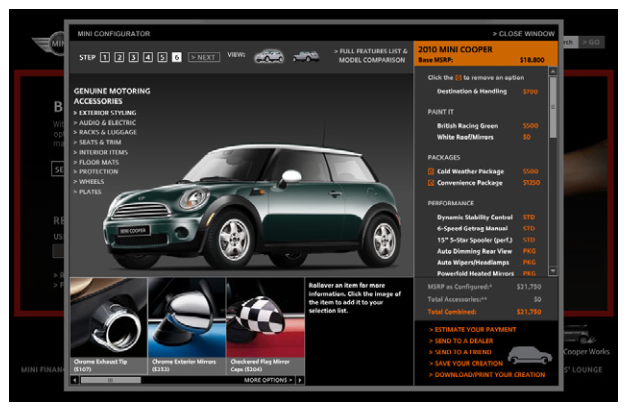
\includegraphics[scale=0.5]{images/lec07-pic44.png}
	\end{figure}
\end{frame}	

\begin{frame}[t]{Breadcrumbs}
	На каждой странице с большим количеством уровней навигационной иерархии, отображайте список всех родительских страниц, вплоть до главной или домашней страницы.
	\begin{figure}[h]
		\centering
		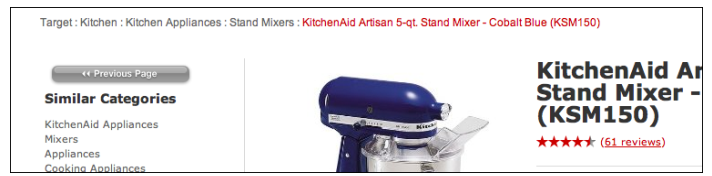
\includegraphics[scale=0.5]{images/lec07-pic45.png}
	\end{figure}
\end{frame}	

\begin{frame}[t]{Breadcrumbs}
	\begin{figure}[h]
		\centering
		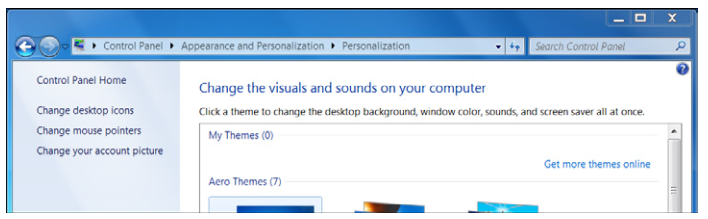
\includegraphics[scale=0.5]{images/lec07-pic46.png}
	\end{figure}
	\begin{figure}[h]
		\centering
		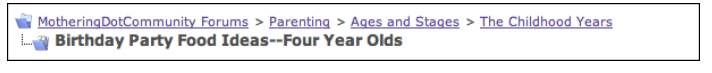
\includegraphics[scale=0.5]{images/lec07-pic47.png}
	\end{figure}	
\end{frame}

\begin{frame}[t]{Annotated Scrollbar}
	Сделайте так, чтобы полоса прокрутки могла бы использоваться в качестве индикатора <<вы здесь>>.
	\begin{figure}[h]
		\centering
		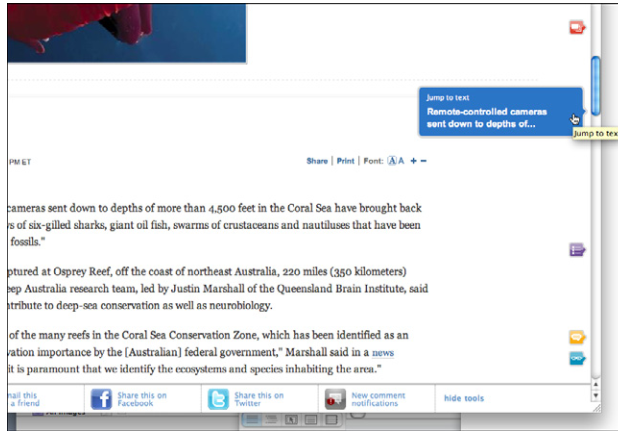
\includegraphics[scale=0.5]{images/lec07-pic48.png}
	\end{figure}
\end{frame}	

%\section{Расположение элементов}
%\section{Действия и команды}
%\section{Формы и элементы управления}

\end{document}
